\documentclass[10pt,a4paper]{report}

\usepackage[table,xcdraw,dvipsnames]{xcolor}
\usepackage{graphicx}
\usepackage{subcaption}
\usepackage[subpreambles=true]{standalone}
\usepackage[utf8]{inputenc}
\usepackage{import}
\usepackage[parfill]{parskip}
\usepackage{float}
%\usepackage[style=numeric-comp,useprefix,hyperref,backend=bibtex]{biblatex}

%Graphics%
\usepackage{pgf}
\usepackage{tikz}
\usetikzlibrary{arrows} % Better Arrow YO
\usepackage{makecell}%

% Changes identation to suit english language
\usepackage[english]{babel}

% Links on the table of contents
\usepackage{hyperref}
\hypersetup{
    colorlinks,
    citecolor=black,
    filecolor=black,
    linkcolor=black,
    urlcolor=black
}

% To eventually print raw text
\usepackage{verbatim}

% Eventual math formulas
\usepackage{amsfonts}
\usepackage{amsmath}
\usepackage{amssymb}

% To Print code
\usepackage{listings}
\lstset{xleftmargin=.2\textwidth, xrightmargin=.2\textwidth}

%table
\usepackage{booktabs}
\usepackage[table,xcdraw]{xcolor}

\usepackage[usenames,dvipsnames]{pstricks}
\usepackage{pstricks-add}
\usepackage{epsfig}
\usepackage{pst-grad} % For gradients
\usepackage{pst-plot} % For axes
\usepackage[space]{grffile} % For spaces in paths
\usepackage{etoolbox} % For spaces in paths
\makeatletter % For spaces in paths
\patchcmd\Gread@eps{\@inputcheck#1 }{\@inputcheck"#1"\relax}{}{}
\makeatother

\author{Libè Jacopo, Guglielmetti Kevin}
\title{RASD Baseline}
\pagestyle{headings}

\begin{document}
    %\pagenumbering{gobble}
    
%TITLE PAGE%
\begin{titlepage}
    \centering
    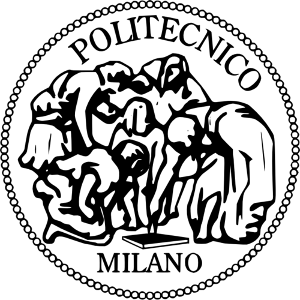
\includegraphics[width=0.35\textwidth]{images/logo_poli.png}\par\vspace{1cm}
    {\scshape\LARGE Politecnico di Milano \par}
    \vspace{1cm}
    {\scshape\Large Appunti \par}
    \vspace{1.5cm}
    {\huge\bfseries Game Theory\par}
    \vspace{2cm}
    {\Large\itshape Libè Jacopo\par}
    \vfill
    {\large \today\par}
\end{titlepage}
    \tableofcontents

    \chapter{Introduction}
        \newpage
        
        
        %DA SISTEMARE%
        Game theroy handles both deterministic and probabilistic games.
        I giochi non cooperative permettono di comunicare ma nessuno accordo tra player è garantito.
        \section{Players}
        I giocatori sono Selfish non nel senso letterale, ma nelle proprie intenzioni.

        In termini matematici (accennando ai prossimi capitoli), definita una utility function $u(x)$ che indica la preferenza di Player 1.
        Le scelte di Player 1 sono sempre volte a massimizzare $u(x)$.

        \section{Preferences}
        X è il set dei risultati del gioco, dato un risultato x devo poterlo confrontare con altri risultati appartenenti a X. Devo quindi avere un operatore di preferenza "$\succeq$" tra elementi del set.

        Per definire le preferenze su elementi del set X si può definire una Utility Function
        
        $u: X \to \Re \hspace{.25cm} tc. \hspace{.25cm} u(x) \ge u(y) \implies x \succeq y$

        Abbiamo bisogno di questa funzione soprattutto se alcune mosse del gioco dipendono dalla probabilità.
        In ogni caso è comunque più semplice lavorare con delle utility function perchè ovviamente lavoriamo in $\Re$

        \section{Beauty Contest con numeri}
        Se scelgo un numero devo sceglierlo sotto la media, quindi < 50.
        Ma se tutti scelgono sotto il 50 allora la media sarà 25, continuando il ragionamento l'unico numero possibile da scegliere razionalmente è il più piccolo dei numeri.

        \section{Bi-Matrix Games}
        Alcuni giochi possono essere rapresentati sotto forma di bimatrice, ovvero ogni cella è un vettore delle utility functions dell'i-esimo giocatore.
        Ad ogni player è permessa la scelta si una riga/colonna su un asse. Ogni player deve scegliere la sua scelta migliore per cui la utility è migliore.
        
        Un gioco viene quindi rappresentato così, con $x_{ij}$ la cella causata da:
        \begin{itemize}
            \item Player 1 sceglie $i$ (strategie su Righe)
            \item Player 2 sceglie $j$ (strategie su Colonne)
        \end{itemize}
        e $u_n(x_{ij})$ la utility function del Player $n$
        \begin{center} 
        $
        \begin{bmatrix}
            (u_{1}(x_{11}),u_{2}(x_{11})) & (u_{1}(x_{12}),u_{2}(x_{12})) \\
            (u_{1}(x_{21}),u_{2}(x_{21})) & (u_{1}(x_{22}),u_{2}(x_{22})) 
        \end{bmatrix}
        $
        \end{center}
    \chapter{Games in Extensive Form}
        \section{Perfect Information Games}
        Un gioco è detto con \textbf{perfect information} quando ogni player conosce la storia degli eventi accaduti e sa in che stato si trova il gioco.
        
        \section{Parties Game}
        Questo gioco ha 4 possibili risultati (ordinati per utility):
        \begin{itemize}
            \item[\textbf{4}] voto no, ottengo aumento
            \item[\textbf{3}] voto si, ottengo aumento
            \item[\textbf{2}] voto no, non ottengo aumento
            \item[\textbf{1}] voto si, non ottengo aumento   
        \end{itemize}

        Possiamo rappresentare tutte le scelte del gioco sapendo che ogni politico sa cosa hanno fatto gli altri.
        Creo così un albero con radice il primo politico e rami le scelte possibili (si, no). Ogni child rappresenta il politico (n+1)-esimo sapendo che quelli prima di lui hanno effettuato un certo numero di scelte (percorso effettuato).
        Le foglie dell'albero sono i vettori delle utility function per ogni politico in base al percorso scelto.

        Ogni livello è un giocatore, più un giocatore si trova lontano dall'origine e più ha strategie disponibili.
        Disegnare un albero del genere però diventa molto velocemente difficile.

        \section{Chance Game (Lancio della Moneta)}
        Ho due giocatori che possono decidere se giocare o no insieme, se uno dei due decide di non giocare il gioco finisce.
        Se entrambi decidono di giocare lancio una moneta per decidere chi ha vinto.

        3 possibili risultati (espressi come vettore utility):
        \begin{itemize}
            \item[\textbf{(0,0)}] I player non decidono di giocare
            \item[\textbf{(1,-1)}] Player 1 Vince, 2 Perde
            \item[\textbf{(-1,1)}] Player 2 Vince, 1 Perde
        \end{itemize}
        I 2 player nell'albero possono scegliere (in ordine) se giocare o se mollare.
        Nell'albero devo introdurre un player fasullo, il "caso" le cui scelte hanno associato una probabilità. In questo caso 50:50.

        Dal punto di vista matematico, il layer "R" può essere rimosso e sostituito con la risoluzione 0. Non importa se gioco o meno, il risultato è lasciato al caso non ho modo di dire quale risultato è assicurato.

        Da questo esempio posso notare anche che una utility function potrà anche tenere conto del rischio associato ad una scelta e non solo del risultato possibile. (Ad esempio potrebbe interessarmi di più vincere 1M€ con 1 lancio invece che 2M€ con 2 lanci).

        \section{Formal Definition}
        La forma estesa di un gioco è un albero. (Le slide per rispasso definiscono le più generiche definizioni di grafo, grafo direzionato e grafo orientato)
        
        Un albero è un grafo orientato dove esiste un nodo $x_{0}$ da cui esiste uno e un solo percorso tra $x_{0}$ e $x_{i}$ con $x_{0},x_{i} \in  V$

        Per la rappresentazione di un gioco dobbiamo però introdurre alcune condizioni addizionali.
        Slide 8-9 del set 2 per queste assunzioni. 
        
        Per "partition" $P_{i}$ si intende un gruppo di vertici. In questo caso non hanno intersezione ($\forall i,j | i \neq j, P_{i} \cap P_{j} = \emptyset$), e una partizione $P_{i}$ rappresenta una sezione orizzontale di vertici appartenenti al player $i$-esimo.
        
        L'ultima partizione $P_{n+1}$ è la partizione dei nodi affidati al caso, può non esistere.
        
        \textbf{NB}: Quando $P_{n+1} \neq \emptyset$ allora ogni nodo ha bisogno di una utility function. Se invece è vero non è necessaria.

        \section{Solving the Game}
        Se utilizziamo le assunzioni sulla razionalità che abbiamo introdotto allora un gioco espresso in forma estesa avrà un solo risultato razionale.
        (Se non c'è casualità)

        Utilizziamo la \textbf{backward-induction}, partendo dai nodi foglia.

        Considerando il layer $i+1$, so che sto considerando le scelte del Player $i$-esimo, quindi per ogni foglia scelgo la scelta che produce l'utility migliore per il player $i$ per ogni set di scelte possibili.

        Procedo al layer superiore fissando la scelta effettuata dal player $i$-esimo.

        Continuo fino ad arrivare al Player 1.

        Scelto il percorso iniziato da Player 1, seguo le scelte migliori per ogni Player per ottenere le scelte del \textbf{percorso razionale}.

        Abbiamo ancora un problema, le foglie possono essere lontanissime dall'origine e in molti giochi difficilmente trovabili.

        \textbf{Oss} se un player ha la stessa utility tra due scelte, allora posso sostituire il player con un nodo affidato al caso con una probabilità uniforme di scegliere una delle sue scelte migliori.

        Quindi la backward-induction non sempre ci offre una soluzione deterministica.

        \section{Esempio Notevole (Centipe Game)}
        % \usepackage[usenames,dvipsnames]{pstricks}
% \usepackage{epsfig}
% \usepackage{pst-grad} % For gradients
% \usepackage{pst-plot} % For axes
% \usepackage[space]{grffile} % For spaces in paths
% \usepackage{etoolbox} % For spaces in paths
% \makeatletter % For spaces in paths
% \patchcmd\Gread@eps{\@inputcheck#1 }{\@inputcheck"#1"\relax}{}{}
% \makeatother
% % User Packages:
% 
% 

\psscalebox{1.0 1.0} % Change this value to rescale the drawing.
{
\begin{pspicture}(0,-3.93125)(12.56,3.93125)
\definecolor{colour0}{rgb}{0.0,0.0,0.0}
\definecolor{colour1}{rgb}{0.19607843,1.0,0.19607843}
\psdots[linecolor=black, dotsize=0.4](1.6,3.3536522)
\psdots[linecolor=black, dotsize=0.4](3.2,2.1536524)
\psdots[linecolor=black, dotsize=0.4](4.8,0.9536523)
\psdots[linecolor=black, dotsize=0.4](6.4,-0.24634765)
\psdots[linecolor=black, dotsize=0.4](8.0,-1.4463477)
\psdots[linecolor=black, dotsize=0.4](9.6,-2.6463478)
\rput[bl](2.0,3.7536523){1}
\rput[bl](3.2,2.5536523){2}
\rput[bl](4.8,1.3536524){1}
\rput[bl](6.4,0.15365234){2}
\rput[bl](8.0,-1.0463476){1}
\rput[bl](9.6,-2.2463477){2}
\rput[bl](10.4,-3.8463476){(1000,1000)}
\rput[bl](6.8,-3.8463476){(102,1001)}
\rput[bl](5.6,-2.6463478){(103,99)}
\rput[bl](4.4,-1.4463477){(3,100)}
\rput[bl](3.2,-0.24634765){(4,1)}
\rput[bl](1.6,0.9536523){(0,2)}
\rput[bl](0.0,2.1536524){(1,1)}
\psline[linecolor=black, linewidth=0.04](1.6,3.3536522)(3.2,2.1536524)
\psline[linecolor=black, linewidth=0.04](3.2,2.1536524)(4.8,0.9536523)
\psline[linecolor=black, linewidth=0.04](4.8,0.9536523)(6.4,-0.24634765)
\psline[linecolor=black, linewidth=0.04](6.4,-0.24634765)(8.0,-1.4463477)
\psline[linecolor=black, linewidth=0.04](1.6,3.3536522)(0.8,2.5536523)(0.8,2.5536523)
\psline[linecolor=black, linewidth=0.04](3.2,2.1536524)(2.4,1.3536524)
\psline[linecolor=black, linewidth=0.04](4.8,0.9536523)(4.0,0.15365234)
\psline[linecolor=black, linewidth=0.04](6.4,-0.24634765)(5.6,-1.0463476)
\psline[linecolor=black, linewidth=0.04](8.0,-1.4463477)(7.2,-2.2463477)(7.2,-2.2463477)
\psline[linecolor=black, linewidth=0.04](8.0,-1.4463477)(9.6,-2.6463478)(8.8,-3.4463477)
\psline[linecolor=black, linewidth=0.04](9.6,-2.6463478)(10.4,-3.4463477)
\psframe[linecolor=colour0, linewidth=0.04, strokeopacity=0.0, fillstyle=solid,fillcolor=colour1, opacity=0.39607844, dimen=outer](8.8,-3.4463477)(6.8,-3.8463476)
\psframe[linecolor=colour0, linewidth=0.002, strokeopacity=0.0, fillstyle=solid,fillcolor=colour1, opacity=0.39607844, dimen=outer](7.2,-2.2463477)(5.6,-2.6463478)
\psframe[linecolor=colour0, linewidth=0.002, strokeopacity=0.0, fillstyle=solid,fillcolor=colour1, opacity=0.39607844, dimen=outer](5.6,-1.0463476)(4.4,-1.4463477)
\psframe[linecolor=colour0, linewidth=0.002, strokeopacity=0.0, fillstyle=solid,fillcolor=colour1, opacity=0.39607844, dimen=outer](4.0,0.15365234)(3.2,-0.24634765)
\psframe[linecolor=colour0, linewidth=0.002, strokeopacity=0.0, fillstyle=solid,fillcolor=colour1, opacity=0.39607844, dimen=outer](2.4,1.3536524)(1.6,0.9536523)
\psframe[linecolor=colour0, linewidth=0.002, strokeopacity=0.0, fillstyle=solid,fillcolor=colour1, opacity=0.39607844, dimen=outer](0.8,2.5536523)(0.0,2.1536524)
\end{pspicture}
}

        \section{Exercises 20 September}
        \subsection{Exam Bonus}
            Give me 1 point or give my colleague 3 points. Both players need to chose without comunication.

        \begin{center} 
            $
            \begin{bmatrix}
                (1,1) & (0,4) \\
                (0,4) & (3,3)
            \end{bmatrix}
            $
        \end{center}

        The result is TOP,RIGHT

        \subsection{Cops and Robbers}
        $
        \begin{matrix}
              &     A  &     B  &     C  &     D  &     E  &     F      \\
            A & (1,-1) & (1,-1) & (1,-1) & (-1,1) & (-1,1) &            \\
            B & (1,-1) & (1,-1) & (1,-1) & (-1,1) & (-1,1) &            \\
            C & (1,-1) & (1,-1) & (1,-1) & (1,-1) & (-1,1) &            \\
            D & (-1,1) & (1,-1) & (-1,1) & (1,-1) & (1,-1) &            \\
            E & (1,-1) & (1,-1) & (1,-1) & (-1,1) & (-1,1) &            \\
            F & (1,-1) & (1,-1) & (1,-1) & (-1,1) & (-1,1) &            \\
        \end{matrix}
        $

        A e B non sono mai scelte dalla guardia

        \subsection{Rock, Paper, Scissors}
        $
        \begin{matrix}
              &        &   1/3  &   1/3  &   1/3  \\
              &        &     R  &     P  &     S  \\
         1/3  &      R & (0,0)  & (-1,1) & (1,-1) \\
         1/3  &      P & (1,-1) & (0,0)  & (-1,1) \\
         1/3  &      S & (-1,1) & (1,-1) & (0,0)  \\
        \end{matrix}
        $

        \textbf{NBB} Se uno dei giocatori sa che l'altro ha una probabilità non uniforme può variare la proria mossa per sfruttarne il vantaggio. (Moltiplico la probabilità del player conosciuto per la mia utility)

        \subsection{Take Away Game}
        Posso determinare quali sono le posizioni di perdita certe:
        \begin{itemize}
            \item [1] Win
            \item [2] Win
            \item [3] Lose
            \item [4] Win
            \item [5] Win
            \item [6] Lose
            \item ....
        \end{itemize}
        La strategia è quella di portarmi ad un multiplo di 3.

        \subsection{Taxi Ride}
        Per modellizare questo problema devo procedere nello stesso modo di prima, trovare una situazione stabile in cui alcun player può rifiutare.
        Ovviamente la scelta migliore sarebbe andare tutti insieme per 20€ e dividere tra i 3. Se questa divisione rispetta i vincoli di andare da soli a tutti converrà andare insieme.

        Pongo quindi come condizione $X_A + X_B + X_C = 20$

        Dai vincoli del gioco conosco che 
        \begin{itemize}
            \item $X_A \le 10$
            \item $X_B \le 10$
            \item $X_C \le 14$
            \item $X_A + X_B \le 12$
            \item $X_A + X_C \le 18$
            \item $X_B + X_c \le 18$
        \end{itemize}

        Risolvendo il vincolo trovo (4,4,12)

        Chiedere al Kex per le funzioni
        
        \subsection{Stock Holders}
        L'obbiettivo è ottenere il 51\% delle share. A è dominante (ha bisogno solo dell'1\% e non è disposto a cedere quote).

        Le condizioni di vittoria/perdita per A sono 
        \begin{itemize}
            \item $v(A \cup B) = W$
            \item $v(A \cup C) = W$
            \item $v(A \cup B \cup C) = W$
            \item $v(A) = L$
        \end{itemize}

        Le condizioni di vittoria/perdita per B e C sono 
        \begin{itemize}
            \item $v(B \cup A) = W$
            \item $v(B \cup C) = W$
            \item $v(B \cup A \cup C) = W$
            \item $v(B) = L$
        \end{itemize}

        Noto che però B/C hanno lo stesso potere. A è dominante.

        \subsection{Pollution Game}
        E' un semplice esempio che fa vedere quanto sia controproducente un gioco non cooperativo.

        \subsection{Sharing Bandwidth}
        Proposta: se scelgo un numero inferiore a $1/n$, e gli altri player sono razionali ho buttato $1/n - x_i$ di banda.
        Se scelgo un numero maggiore di $1/n$ e tutti gli altri player sono razionali allora nessuno ha banda e il canale di chiude.
        La scelta razionale è scegliere $1/n$.

        \subsection{Missing Lessons...}

        \subsection{Non Cooperative Games}
        La rappresentazione Bi-Matriciale dei giochi non cooperativi va bene ma è limitata dal fatto che assume un numero definito di strategie per i player.
        Una definizione più formale e generale è quella presentata sulle slide.

        \begin{center}
            $X,Y,f: X \times Y \rightarrow \mathbb{R}, g: X \times Y \rightarrow \mathbb{R} $
        \end{center}

        Dove $X,Y$ sono i set delle decisioni per i player X e Y. E $f,g$ sono le loro utility function.
        
        Un player può avere delle "mixed strategies" ovvero, se le strategie di un player sono per esempio:
        \begin{center}
            $m \in \mathbb{N} {x_1,x_2,\dots,x_m}$
        \end{center}

        Possiamo definire un set di $m$ probabilità che soddisfa certe proprietà detto \textbf{simplex}:
        \begin{center}
            $p_i \ge 0$

            $\sum_{i = 1}^{m} p_i = 1$ 
        \end{center}

        \subsubsection{Esempio}
        Se abbiamo un problema definito come:

        $X,Y: dim(X)=m, dim(X)=n$  $f,g$  $X,Y \text{finite}$

        Possiamo costruire un nuovo gioco con le mixed strategies:

        $\hat{X}, \hat{Y}$  $\hat{f}, \hat{g}$ $\hat{X}, \hat{Y} \text{finite}$

        dove 
        
        $\hat{X}$ è un simplex $m$-dimensionale

        $\hat{Y}$ è un simplex $n$-dimensionale

        Ma cosa sono ora $\hat{f}, \hat{g}$? Sono le \textbf{expected-utility}. 
        
        Come le calcoliamo però? Dobbiamo pesare le utility esistenti.

        \subsubsection{Realizzazione Esempio}
        $X={T,B} Y={L,R}$

        La bimatrice è
        \begin{center} 
            $
            \begin{matrix}
                & L & R \\
                T & (u_{LT}^1,u_{LT}^2) & (u_{RT}^1,u_{RT}^2) \\
                B & (u_{LB}^1,u_{LB}^2) & (u_{RB}^1,u_{RB}^2)
            \end{matrix}
            $
        \end{center}

        $\hat{X}=[0,1], 0 \le p \le 1$
        
        $\hat{Y}=[0,1], 0 \le q \le 1$

        Quindi per Y le probabilità pesate sono $Lq, R(1-q)$

        Possiamo calcolare le expected utility pesandole:
        
        $\hat{f}(p,q)= pqu_{LT}^1 + p(1-q)u_{RT}^1 + (1-p)qu_{BL}^1 + (1-p)(1-q)u_{BR}^1$
        
        $\hat{g}(p,q)= pqu_{LT}^2 + p(1-q)u_{RT}^2 + (1-p)qu_{BL}^2 + (1-p)(1-q)u_{BR}^2$

        \subsubsection{Conclusione}

        Possiamo quindi dedurre che dato un qualsiasi gioco con strategie pure possiamo costruirne uno con strategie miste.
        
        \subsection{Esempio Caso n-dimensionale mixed-strategy}
        \begin{center}
            $X,Y,f: X \times Y \rightarrow \mathbb{R}$

            $\text{dim}(X)=m$

            $\text{dim}(Y)=n$
        \end{center}

        Rappresentando i simplex e le expected-utility:

        $\hat{X},\hat{Y}$ $p \in \hat{X} p=\{p_1,\dots,p_m\}$ $p_i \ge 0$ $\sum p_i = 1$

                          $p \in \hat{X} p=\{p_1,\dots,p_m\}$ $p_i \ge 0$ $\sum p_i = 1$

                $\sum_{j = 1,n\\i=1,m} f(x_i,y_j) = \hat{f}(p,q)$  

        Rappresentando le bimatrici:

        $B,A \in M \times N$  $A_{ij} = f(x_i,y_j)$ 
                              $B_{ij} = g(x_i,y_j)$

        $p,q: p^T\underline{A}q = \begin{bmatrix}
                                        p_1 & p_2 & \dots & p_n
                                    \end{bmatrix}
                                    \begin{bmatrix}
                                        A_{11} & \dots & A_{1n} \\
                                        \dots & \dots & \dots \\
                                        A_{m1} & \dots & A_{mn}
                                    \end{bmatrix}
                                    \begin{bmatrix}
                                        q_1 \\ q_2\\ \dots \\ q_n
                                    \end{bmatrix}$ 
        
        $q = \begin{bmatrix}
                q_1 \\ q_2\\ \dots \\ q_n
            \end{bmatrix}, p = \begin{bmatrix}
                                p_1 \\ p_2\\ \dots \\ p_n
                            \end{bmatrix}$


        \chapter{Nash Equilibrium}

        \subsection{Definition}
        E' una combinazione di due condizioni:
        \begin{itemize}
            \item P1 non può migliorare la sua scelta data una scelta da P2
            \item P2 non può migliorare la sua scelta data una scelta da P1
        \end{itemize}

        In altre parole è una combinazione di strategie \textbf{stabile} rispetto alle decisioni di un singolo player.
        Ogni player non ha motivo di scegliere altre opzioni.

        Posso notare che è una versione più forte della definizione di \textbf{(weakly) dominant strategy} che ricordo essere:
        \begin{center}
            $f(\overline{x}, y) \ge f(x,y) \forall x,y$
        \end{center}

        La definizione di \textbf{Nash-Equilibrium} è infatti:
        \begin{center}
            $f(\overline{x}, \overline{y}) \ge f(x,\overline{y}) \forall x$
        \end{center} 

        \subsubsection{Osservazione}

        Se $\overline{x}$ è una scelta dominante, allora se esiste un valore $\overline{y}$ che massimizza $g(\hat{x}, y)$ allora $(\overline{x}, \overline{y})$ è un equilibrio di Nash.

        Questa definizione per quanto utile non può dirci niente nel caso non possa massimizzare la funzione o il player X non sia in posizione dominante.

        \subsection{Execise: Extensive Form to Bi-Matrix}


        % \usepackage[usenames,dvipsnames]{pstricks}
% \usepackage{epsfig}
% \usepackage{pst-grad} % For gradients
% \usepackage{pst-plot} % For axes
% \usepackage[space]{grffile} % For spaces in paths
% \usepackage{etoolbox} % For spaces in paths
% \makeatletter % For spaces in paths
% \patchcmd\Gread@eps{\@inputcheck#1 }{\@inputcheck"#1"\relax}{}{}
% \makeatother
% % User Packages:
% 
% 

\psscalebox{1.0 1.0} % Change this value to rescale the drawing.
{
\begin{pspicture}(0,-2.93125)(8.04,2.93125)
\psdots[linecolor=black, dotsize=0.4](4.4,2.3536522)
\psdots[linecolor=black, dotsize=0.4](2.0,-0.84634763)
\psdots[linecolor=black, dotsize=0.4](6.4,-0.84634763)
\psline[linecolor=black, linewidth=0.04](4.4,2.3536522)(2.0,-0.84634763)
\psline[linecolor=black, linewidth=0.04](4.4,2.3536522)(6.4,-0.84634763)
\psline[linecolor=black, linewidth=0.04](6.4,-0.84634763)(5.2,-2.4463477)
\psline[linecolor=black, linewidth=0.04](6.4,-0.84634763)(7.6,-2.4463477)
\psline[linecolor=black, linewidth=0.04](2.0,-0.84634763)(0.4,-2.4463477)(2.0,-0.84634763)(2.8,-2.4463477)
\rput[bl](0.4,-1.2463477){a}
\rput[bl](2.8,-1.6463476){b}
\rput[bl](5.6,-1.2463477){c}
\rput[bl](7.6,-1.6463476){d}
\rput[bl](6.8,-0.84634763){2}
\rput[bl](5.6,1.1536523){B}
\rput[bl](2.8,0.75365233){T}
\rput[bl](1.6,-0.44634765){2}
\rput[bl](4.4,2.7536523){1}
\rput[bl](0.0,-2.8463476){(1,1)}
\rput[bl](2.4,-2.8463476){(2,1)}
\rput[bl](4.8,-2.8463476){(3,1)}
\rput[bl](7.2,-2.8463476){(2,3)}
\end{pspicture}
}

        $\Rightarrow
        \begin{bmatrix}
              & ac & ad & hc & hd \\
            T & (1,1) & (1,1) & & \\
            B & & & & 
        \end{bmatrix}
        $

        Al contrario:

        $
        \begin{bmatrix}
              & L & R \\
            T & & \\
            B & & 
        \end{bmatrix}
        \Rightarrow$
        % \usepackage[usenames,dvipsnames]{pstricks}
% \usepackage{epsfig}
% \usepackage{pst-grad} % For gradients
% \usepackage{pst-plot} % For axes
% \usepackage[space]{grffile} % For spaces in paths
% \usepackage{etoolbox} % For spaces in paths
% \makeatletter % For spaces in paths
% \patchcmd\Gread@eps{\@inputcheck#1 }{\@inputcheck"#1"\relax}{}{}
% \makeatother
% % User Packages:
% 
% 

\psscalebox{1.0 1.0} % Change this value to rescale the drawing.
{
\begin{pspicture}(0,-2.0987988)(6.814142,2.0987988)
\psdots[linecolor=black, dotsize=0.4](3.6,1.5212011)
\psline[linecolor=black, linewidth=0.04](3.6,1.5212011)(2.0,-0.47879884)
\psline[linecolor=black, linewidth=0.04](3.6,1.5212011)(5.2,-0.47879884)
\psline[linecolor=black, linewidth=0.04, linestyle=dashed, dash=0.17638889cm 0.10583334cm](2.0,-0.47879884)(5.2,-0.47879884)
\psline[linecolor=black, linewidth=0.04](2.0,-0.47879884)(0.4,-2.0787988)(0.4,-2.0787988)
\psline[linecolor=black, linewidth=0.04](2.0,-0.47879884)(2.4,-2.0787988)
\psline[linecolor=black, linewidth=0.04](5.2,-0.47879884)(4.8,-2.0787988)
\psline[linecolor=black, linewidth=0.04](5.2,-0.47879884)(6.8,-2.0787988)
\rput[bl](0.0,-1.2787988){L}
\rput[bl](2.4,-1.2787988){R}
\rput[bl](4.8,-1.2787988){L}
\rput[bl](6.4,-1.2787988){R}
\rput[bl](2.4,0.32120118){T}
\rput[bl](4.8,0.7212012){B}
\rput[bl](3.6,1.9212012){1}
\rput[bl](4.0,-0.07879883){2}
\end{pspicture}
}


        Noto che la rappresentazione bimatriciale perde informazioni rispetto all'albero esteso

        \subsection{Multi-Function and AvgMax function definition}

        Una multi-function come risultato ha un subset di valori del codominio.

        $x \mapsto f(x) \subset Y$ 

        \textbf{AvgMax} è una multi-funzione che restituisce tutti i massimi (assoluti??) della funzione.

        \subsection{Best-Reply Multifunction}

        La Best-Reply multifunction può essere definita così:

        $\text{BR}_1: Y \rightarrow X : \text{BR}_1(y)=\text{ArgMax}\{f( \bullet , y )\}$

        Ovvero, se player 2 sceglie $y$ allora $\text{BR}_1(y)$ mi da la migliore strategia data quella di player 2.

        Ovviamente abbiamo una definizione simmetrica per player 1.
        \subsubsection{Nuova definizione di Equilibrio di Nash}

        $(\overline{x}, \overline{y})$ è un equilibrio sse $(\overline{x}, \overline{y}) \in \text{BR}(\overline{x}, \overline{y})$

        \subsection{Nash Theorem}

        \textbf{Ipotesi}:
        \begin{itemize}
            \item I set delle strategie devono essere \textbf{convessi}, questo implica che i giochi con decisioni finite non possono essere soggette a questo teorema.
                
                \textbf{Il teorema di Nash non si applica a giochi con strategie pure}
            \item Le utility function devono essere continue
            \item Le utility function devono mappare a set \textbf{quasi concavi}
        \end{itemize}
        
        \textbf{Tesi}: esiste almeno un equilibrio di Nash.

        Dove un set \textbf{convesso} significa che prendendo due elementi e unendoli con una linea, la linea deve essere contenuta nell'insieme in tutti i suoi punti.

        Una funzione \textbf{quasi-concava} è una funzione che data una linea tutto ciò che è sotto la linea è un set convesso.

        Molto spesso abbiamo uno di questi casi:
        \begin{itemize}
            \item Troppi equilibri
            \item Equilibri troppo complicati da computare
            \item Nessun equilibrio
        \end{itemize}

        \subsubsection{Corollary}
        Le mixed strategies hanno sempre almeno un equilibrio di Nash. (Il prof pensava di averlo già fatto e lo ha saltato velocemente)

        \subsection{Exercise: Finding Nash equilibria (Bi-Matrix)}
        $
        \begin{matrix}
            & L & R \\
            T & (1,0) & (0,3) \\
            B & (0,2) & (1,0) 
        \end{matrix}
        $

        Per prima cosa calcola la "expected-utility", so che le probabilità per scelta sono:

        Player 1: $\begin{matrix}
            T & B \\
            (p, & 1-p)
        \end{matrix}$

        Player 2: $\begin{matrix}
            L & R \\
            (q, & 1-q)
        \end{matrix}$

        Le utility sono quindi:
        
        Considerando le utility di player 1 e le probabilità:

        $\begin{bmatrix}
            & L(q) & B(1-q) \\
            T(p) & 1 & 0 \\
            B(1-p) & 0 & 1
        \end{bmatrix} \Rightarrow $
        
        Otteniamo quindi:

        $f(p,q)= pq + (1-p)(1-q) = p(2q-1)-q+1$

        Per P2:

        $\begin{bmatrix}
            & L(q) & B(1-q) \\
            T(p) & 0 & 3 \\
            B(1-p) & 2 & 0
        \end{bmatrix} \Rightarrow $

        $g(p,q)= 3p(1-q) + 2(1-p)q = q(2 - 5p) + 3p$

        Ora calcolo le scelte migliori (dato $q$ voglio massimizzare $p$):

        \subsubsection{BR Player 1}
        $p(2q-1)$ posso cambiarlo (posso scegliere p), la parte invece $-q+1$ non posso toccarla come Player 1 quindi la ignoro.

        Studio quindi la prima parte:

        $2q-1 < 0, q < 1/2, p=0$

        $2q-1 = 0, q = 1/2, p \in [0,1]$

        $2q-1 > 0, q > 1/2, p=1$

        Se P2 ha $0 \le q < 1/2$ allora il valore della prima parte sarebbe negativo quindi per contrastare P1 deve imporre $p=0$.

        Se P2 ha $q = 1/2$ allora P1 può avere qualsisi valore di $p \in [0,1]$ e non cambierà nulla (la prima parte di azzera).

        Se P2 ha $q > 1/2$ allora P1 è avantaggiato (prima parte positiva) e quindi per massimizzare il guadagno deve porre $p=1$.

        La stessa cosa si può fare per P2.

        Plottando le due best strategy posso trovare un punto di equilibrio.

        \subsubsection{Osservazione}
        Se uno dei due giocatori sceglie di giocare una strategia di equilibrio, cosa sceglie l'altro giocatore non cambia la situazione.

        Per questo motivo il teorema è anche detto il teorema dell'indifferenza.

        \section{N-Player Games}
        Ci sono $n$ giocatori, ogni player ha il proprio set di strategie $X_i$ e di "payoff" (utility) $f_i: X \rightarrow \mathbb{R}$ con $X = \prod_{j=1}^nX_j$

        \subsection{}{Nash Equilibrium for n-players}

        La definizione vettoriale di un equilibrio di Nash è:

        $\overline{x} \hspace{.5cm} f_i(\overline{x}_i, \overline{x}_{-i}) \ge f_i(x, \overline{x}_{-i}) \hspace{.5cm} \forall x  \in X_i \hspace{.5cm} \forall i$

        Dove $\overline{x}$ è il vettore delle strategie e $\overline{x}_{-i}$ è il vettore della strategie meno quelle del player $i$.


        \section{Congestion Games}

        I giocatori vogliono muoversi da un punto ad un altro, devono seguire alcune regole e più persone ci sono nel gioco e più si va lenti.

        L'obbiettivo è quello di distribuire i player sulle strade in modo da ottimizzare il traffico.

        Abbiamo quindi
        \begin{itemize}
            \item $N$ giocatori
            \item Il set delle risorse $R$ (strade, etc.)
            \item Una collezione di sottoinsiemi di $R$ (le strategie)
            \item Per ogni $r$ risorsa abbiamo $d_r: \mathbb{N} \rightarrow \mathbb{R}$ (la funzione costo di utilizzo di $r$)
        \end{itemize}

        Il costo di una risorsa dipende dal numero di giocatori che la usano.

        \subsection{Braess Paradox}

        La situazione senza paradosso è la seguente:

        Si può vedere che vi sono 2 percorsi A e B. E Sono simmetrici, quindi ho moltissimi equilibri di Nash che però prevedono 2000 player su A e 2000 su B.

        Quando sono in equilibrio allora il percorso su A e B è uguale per entrambi i percorsi a 20 minuti.

        $A = 2000/400 + 15 = 20 \text{minuti}$

        $B = 15 + 2000/400 = 20 \text{minuti}$

        Abbiamo molti equilibri perchè ho tutte le permutazioni dei 2000 player su A e B.

        \subsubsection{Paradosso}

        Assumiamo di aprire una strada con costo 2 tra A e B (a metà).

        Noto che non ho più lo stesso equilibrio, all'inizio sembrerebbe che facendo i segmenti $N/400$ infatti usando la condizione di prima:

        $\frac{2000}{400} + 2 + \frac{2000}{400} = 12$ minuti.

        Ma questa situazione non è di equilibrio, tutti vorranno andare su quella strada. Quindi l'equilibrio ora prevede che tutti 4000 passino per i segmenti $\frac{N}{400}$.

        Il nuovo equilibrio quindi è $\frac{4000}{400} + 2 + \frac{4000}{400} = 22$ minuti.

        Il paradosso è che aggiungendo una strada ottengo un tempo di percorrenza peggiore.

        \subsection{El Ferol bar (3 people)}

        La parte interessante sta nel calcolo della strategia mix-strategy di equilibrio. \textbf{Nei giochi di congestione solitamente l'equilibrio delle mixed-stratgy è una probabilità uguale per tutti}.

        Calcolo quindi la mia expected utility assumendo che gli altri due player siano andati al bar con probabilità $p$.
        
        La probabilità combinata dei due è quindi $p^2$ e la probabiltà che non sia soccesso è $1-p^2$.

        \subsubsection{Osservazione}
        I giochi di congestione hanno \textbf{sempre} equilibri di Nash (puri) ed asimmetrici.

        \subsection{Duopoly models}
        
        \chapter{Zero-sum Games}
        %Missing Lesson%

        \chapter{Repeated games/Correlated equilibria}
        
        Come abbiamo visto nel problema del prigioniero, l'unico equilibrio di Nash è il peggior risultato per tutti i player.

        Lo scopo di questo capitolo è trovare un'alternativa migliore a questo equilibrio.

        \section{Repeated Games}

        Riportiamo di nuovo il Prisoner's Dilemma

        \begin{center}
            $
            \begin{matrix}
                (3,3) & (0,10) & (-2,-2)             \\
                (10,0) & (1,1) & (-1,-1)             \\
                (-2,-2) & (-1,-1) & (-2,-2)             \\
            \end{matrix}
            $    
        \end{center}
        
        L'equilibrio è (1,1). Ma esiste un equilibrio migliore?

        Cosa succede se giochiamo il gioco per più giorni? Possiamo dimostrare che $\forall a > 0$ se il gioco è giocato abbastanza volte i giocatori ottengono almeno 3.

        Se definiamo due numeri $k$ e $N$, dove $N$ numero di giorni e $k$ è il giorno in cui i player cercano di prendere 10.

        Allora possiamo definire una strategia per cui $N - k$ giorni i player scelgono la prima colonna e i restanti $k$ giorni scelgono il loro 10.

        Notiamo che se cambiano solo all'ultimo giorno la loro utility sarà:

        \begin{center}
            $\frac{(N-k)3 + k1}{N}$
        \end{center}

        Se un player cambia al $k$-esimo giorno diverso dall'ultimo avrà un guadagno medio di:
        \begin{center}
            $\frac{(N-k-1)3 + 10 + k(-1)}{N}$
        \end{center}

        Dove notiamo che un giorno otterrà 10, $k$ giorni in seguito ad aver tradito player 2 verrà punito (e avrà utility -1).

        Notiamo dunque che la strategia proposta sarà un equilibrio solo se il guadagno medio di cambiare l'ultimo giorno sarà maggiore di quello di tradire l'altro player.

        \begin{center}
            $\frac{(N-k)3 + k1}{N} \ge \frac{(N-k-1)3 + 10 + k(-1)}{N}$
        \end{center}

        Che è vero s.s.e $k>3$.

        Essendo un equilibrio posso dimostrare che se i player giocano per un numero sufficientemente alto di giorni, il guadagno medio di ogni player sarà 3.

        \subsubsection{Osservazioni}

        \begin{itemize}
            \item La collaborazione può essere razionalizzata in giochi su più giorni
            \item In questo caso abbiamo trovato un equlibrio di Nash, ma presumiamo che un player tradito sia disposto a punirsi per punire il proprio avversario (abbastanza improbabile).
            \item La ripetizione di un gioco \textbf{cambia} la definizione del gioco.
        \end{itemize}

        \section{Corellated Equilibria}

        Questo equilibrio è invece un'idea diversa di equilibrio rispetto a quello di Nash.

        Per mostrarne la definizione torniamo alla Battle of Sexes.

        \begin{center}
            $
            \begin{matrix}
                (2,1) & (0,0) \\
                (0,0) & (1,2) 
            \end{matrix}
            $    
        \end{center}

        Abbiamo 3 equilibri di Nash:
        $[(1,0)(1,0)][(0,1)(0,1)][(\frac{2}{3},\frac{1}{3})(\frac{1}{3}, \frac{2}{3})]$

        I primi due equilibri sono strategie pure. Il terzo è una mixed strategy ha come risultato $(\frac{2}{3}, \frac{2}{3})$ che però è pessima.

        Perchè? Perchè in questo caso entrambe le scelte sono affidate al caso. E' molto semplice che capitino casi in cui i due vanno in posti diversi.

        In questo caso è abbastanza semplice capire che sarebbe più conveniente giocare più volte il gioco oppure lanciare una moneta per decidere dove andare.

        Cosa succede se correliamo le scelte? Supponiamo di legare la scelta dei due in base al lancio di una moneta. Se testa si va da una parte, se croce dall'altra.

        Notiamo che in questo caso la probabilità sta nella sceltra da i due risultati $(2,1)$ e $(1,2)$, non ci sono casi in cui il risultato è $(0,0)$.

        Nel caso del lancio di una moneta con probabilità $\frac{1}{2}$ abbiamo un guadagno previsto $(\frac{3}{2},\frac{3}{2})$.

        Questo tipo di strategia è detta \textbf{correlated strategy}. In pratica quindi attribuiamo una probabilità alla scelta di un outcome invece che dare una probabilità alle scelte individuali dei player.

        \subsection{Car Crash}

        In questo esempio la scelta è un pò più complicata. Non basta solo una correlated strategy ma anche un'entità che faccia la scelta ed informi i player privatamente.

        Guardare l'esempio sulle slide.

        \subsection{Correlated Equilibria Existence Theorem}

        In soldoni, un equilibrio di Nash genera un Correlated Equilibrio. Un equilibrio di Nash \textbf{è} un correllated equilibria.

        \subsubsection{Osservazione}

        Un \textbf{correlated equilibria} è un'estensione della definizione di equilibrio di Nash.

        \chapter{Cooperative Games}

        In questi giochi se i player decidono di cooperare devono cooperare. In questi giochi tutti conoscono tutto ciò che gli altri faranno.

        Una volta che i player hanno un accordo sono legati a questo accordo.

        Il problema è trovare le coalizioni. Una \textbf{coalition} è un gruppo di giocatori che giocano con un accordo tra loro.

        Un altro problema è trovare le condizioni di ingresso in una coalizione per un player.

        \section{Formal Definition}

        $\mathbb{P}$ è il power-set. Essendo la combinazione di ogni player (l'insieme di tutte le coalizioni possibili) ha cardinalità $2^N$ dove $N$ è il numero di player.

        Solitamente si dice che ha dimensione $2^N -1$ perchè escludiamo la coalizione senza player.

        \textbf{Convenzione}: Quando scriviamo $\mathbb{R}^A$ significa che ho un intero per ogni elemento di $A$.

        \section{Transferable Utility Game}

        La definizione di prima è troppo generica, i TU games sono un sottogruppo di giochi cooperativi.

        Dove ogni coalizione ha una utility assegnata a se $v: 2^N \rightarrow \mathbb{R}$.

        In questo caso quindi valutiamo la coalizione in generale non più la convenienza di ogni player di essere in una coalizione.

        Da questa definizione quindi abbiamo che $V(A) = \{ x \in \mathbb{R}^A : \sum_{i \in A} x_i \le v(A)\}$.

        \subsection{Sellers and Buyer}

        Player 1 è il venditore, e pensa che il suo oggetto valga a.
        Player 2 è un compratore e valuta l'oggetto di P1 con b.
        Player 3 è un compratore e valuta l'oggetto di P1 con c.

        Il problema è posto in modo che $a < b < c$. I venditori valutano l'oggetto di P1 più di quanto è valutato da P1 (sennò non lo venderebbe).

        Abbiamo una serie di coalizioni, quale è la migliore?

        Abbiamo le coalizioni singole, cosa valutano i player senza avere una coalizione? Qua ci perderebbero solo i venditori.

        \begin{center}
            $v(\{1\}) = a, v(\{2\}) = 0, v(\{3\}) = 0$
        \end{center}

        Dopo abbiamo le offerte di acquisto

        \begin{center}
            $v(\{1,2\}) = b$ P1 vende a P2

            $v(\{1, 3\}) = c$ P1 cende a P3

            $v(\{2,3\}) = 0$ P2 non ha nulla da vendere a P3
        \end{center}

        Infine abbiamo la condizione con N player che assume il valore massimo:

        \begin{center}
            $v(N) = c$
        \end{center}

        \subsection{Glove game}

        In questo caso la definizione del gioco è semplice (da non confondere con la definizione di gioco semplice che daremo tra un pò). Ma il problema è chi tra i giocatori avrà più utility degli altri?

        Vediamo subito che P3 è quello che ha più potere, può scegliersi la coalizione gli altri due non hanno potere. L'utility dei singoli player dovrebbe riflettere questo.

        \subsection{Weighted Majority Game}

        Come risolviamo il problema dei votanti UN? 5 membri che devono votare per forza e 10 minoritari di cui ne devono servire 4 per passare un voto.

        Dobbiamo trovare la soglia. E' un gioco semplice.

        Sia $n$ il numero di voti necessari. Avendo 5 maggioritari che devono per forza passare allora $n > (5-1)f(\text{maggioritari} + 10g(\text{minoritari}))$.

        La seconda implica che $n = 5f(\text{maggioritari} + 4g(\text{minoritari}))$

        Se supponiamo $g > 1$ allora $n > (5-1)f + 10$ e $n = 5f + 4$, quindi

        \begin{center}
            $5f + 4 > (5-1)f + 10 \rightarrow f > 6 \rightarrow f = 7, n = 4 \cdot 7 + 4 = 39$
        \end{center}

        \subsection{Peer Game}

        In questo gioco ogni player ha i suoi interessi $v_i$. Esaminando l'albero notiamo condizioni del tipo $v(\{1,2\}) = v(\{1,2, 5\}) = v_1 + v_2$, perchè la coalizione con P5 ha la stessa utility dove $w_5$ non è considerato?
        
        Questo perchè player 5 in quella coalizione non ha potere, il suo peer diretto P3 non fa parte della coalizione.

        \section{The set of TU games}

        Possiamo rappresentare tutti i tipi di giochi TU in un unico gruppo? Si, ogni gioco cooperativo corrisponde ad un vettore.

        Quindi l'insieme di tutti giochi è rappresentabile da un insieme di vettori.

        Ma se abbiamo uno spazio vettoriale possiamo definirne le basi.

        Una di queste basi è composta dagli \textbf{unanimity games}.

        \subsection{Simple Games}

        Possiamo dividere questo set in classi (giochi additivi, superadditivi).

        Una di queste classi è quella dei giochi semplici.

        Ogni costo per coalizione è 0 o 1. La probabilità di avere 1 aumenta all'aumentare della dimensione della coalizione. La coalizione intera ha sempre costo 1.

        \section{Solutions to cooperative games}

        Un vettore soluzione è un vettore contenente le utility dei singoli player.

        Quando parliamo di solution in realtà parliamo di \textbf{solution concept} ovvero non una soluzione specifica ma un modo di trovare una famiglia di soluzioni.

        Una soluzione è un criterio che dato un gioco ci permette di distribuire la utility tra i player.

        \subsection{Imputation}

        Una \textbf{imputation} è una soluzione (una mappa per ogni gioco che fornisce vettori soluzione) fatta in modo che ogni player guadagni più di quanto guadagnerebbe giocando da solo.

        La seconda proprietà è detta \textbf{efficiency} ovvero le i vettori soluzioni datto sempre il valore della coalizione intera.

        \textbf{Oss}. nei giochi additivi o più in generale in tutti i giochi in cui il guadagno della coalizione intera è maggiore di ogni altra coalizione allora ho sicuramente almeno una imputation.

        Se non è un gioco con queste proprietà però può ancora avere una o più imputation (condizione sufficiente).

        \subsubsection{Imputation Set}

        E' il gruppo di tutte le imputation per un gioco particolare. 

        \subsection{The Core}

        Il core è un sottogruppo del gruppo di imputation. Le imputation sono distribuzioni efficienti le cui utility sono migliori di ogni utility individuale. 
        
        Il core è composta da soluzioni efficienti in cui però la somma delle utility di ogni player in una coalizione ha almeno lo stesso guadagno della coalizione stessa.

        Ovvvero le soluzioni nel core sono quelle dove nessuna altra coalizione otterrebbe un valore migliore rispetto alle altre.

        %MISSING LESSON%

        \chapter{Shapley Value and Power Indeces}

        \section{Shapley Theorem}
        $\sigma_i(v)$ è lineare in $v$.

        Il teorema è di \textbf{unicità ed esistenza} di una funzione $\sigma_i(v)$ che ha le proprietà di efficienza, simmetria, null player e additività.

        Ricordiamo che stiamo creando una funzione che funziona per ogni tipo di gioco. Il teorima dice che esiste una funzione $\sigma_i(v)$ che va dal set dei giochi a quello delle utility, quindi deve funzionare per ogni tipo di gioco.

        \subsection{Proof}

        \textbf{[Slide 7]}

        \subsubsection{Efficiency}

        Dobbiamo dimostrare che la somma di tutte le $\sigma_i(v)$ per ogni player deve essere uguale a $v(N)$.

        Per prima cosa consideriamo le coalizioni del tipo $S = N \backslash \{i\}$ otteniamo che il coefficiente è $\frac{(n-1)!(n-n)!}{n!} = \frac{(n-1)! \cdot 1}{n \cdot (n-1)!} = \frac{1}{n}$. 
        
        In seguito consideriamo gli altri tipi di coalizione (ed il nostro obbiettivo è dimostrare che si annullano).

        Dato che rimangono solo i coefficienti per la prima condizione otteniamo che $\sum_{i=1}^n \sigma_i(v) = \sum_{i=1}^n \frac{1}{n} [v(N) - v(N \backslash \{i\})] = n \cdot \frac{1}{n} \cdot v(N) = v(N)$

        \subsubsection{Simmetry}

        Abbastanza dettagliato sulla slide

        \subsubsection{Uniqueness}

        Provate le proprietà, dobbiamo provare l'altra metà del teorema: la unicità della soluzione.

        Se non avessimo la proprietà di unicità, una volta scelte le regole come proposto dalla definizione non potremmo avere un modo per decidere quale è obbiettivamente la divisione migliore.

        In questo caso dimostrare l'unicità è facile.
        
        \textbf{Idea:} assumiamo che abbiamo uno spazio vettoriale $U$ con una base $\{e_i\}$ e che abbiamo una funzione $L_{e_i} = y_i$.
        Sappiamo che essendo $\{e_i\}$ una base posso scrivere ogni vettore $u \in U = \sum_i c_ie_i$. Ma quindi $L_u = \sum_i c_i(L_{e_i}) = \sum_i c_i y_i$.

        Consideriamo ora una base dello spazio dei giochi considerati (unanimity games) $u_A(T) = \big\{ \begin{matrix}
            1, A \subset T \\ 0, \text{otherwise}
        \end{matrix}$.

        La funzione $\phi(u_A) = \{ \begin{matrix}
            \frac{1}{|A|}, i \in A \\
            0, i \notin A
        \end{matrix}$ è unica.??? (ci siamo persi un pezzo)

        \section{Simple Games}

        Definito $A$ come da slide possiamo dire per semplicità che se $A \subset B, u(A) \le u(B)$.

        Se consideriamo $A_i$ la colaizione che non vincerebbe senza il player $i$, allora posso scrivere il valore di Shapley così:

        \begin{center}
            $\sigma_i(v) = \sum_{A \in A_i} \frac{a!(n-a-1)!}{n!}$
        \end{center}

        Alternativamente possiamo scriverla pensando all'insieme $A \in W_i$ delle coalizioni che perdendo il player $i$ rimangono vincenti.

        \begin{center}
            $\sigma_i(v) = \sum_{A \in W_i} \frac{(a-1)!(n-a)!}{n!}$
        \end{center}

        \subsubsection{Esempio}

        \textbf{[Slide 11]}

        Possiamo considerare la tabella per avere un esempio di come calcolare i valori di shapley senza calcolare i coefficienti.

        Sulle colonne abbiamo i contributi del player $i$ che entra nella coalizione sulla colonna. Le righe sono tutti i modi con cui si può formare una coalizione \textbf{compreso l'ordine}.

        Esempio 123 è la coalizione che si forma quando entra 1 per primo, 2 per secondo, 3 per terzo.

        Quindi calcoliamo la prima colonna:

        \begin{tabular}{ |c|c|c|c| }
            \hline
            & 1 & 2 & 3 \\ 
            \hline
            123 & $v(\{1\}) = 0 $ & $v(\{1,2\}) - v(\{1\}) = 4$ & $v(N) - v(\{1,2\}) = 4$  \\
            \hline
            132 & $v(\{1\}) = 0 $ & $v(N) - v(\{1,3\}) = 4$ & $v(\{1,3\}) - v(\{1\}) = 4$  \\
            \hline
            213 & $v(\{1,2\}) - v(\{2\}) = 3$ & $v(\{2\}) = 1 $ & $v(N) - v(\{1,2\}) = 4$  \\
            \hline
            231 & $v(N) - v(\{2,3\}) = 6$ & $v(\{2\}) = 1 $ & $v(\{2,3\}) - v(\{2\}) = 1$  \\
            \hline
            312 & $v(\{1,3\}) - v(\{3\}) = 3$ & $v(N) - v(\{1,3\}) = 4$ & $v(\{3\}) = 1 $  \\
            \hline
            321 & $v(N) - v(\{2,3\}) = 6$ & $v(\{2,3\}) - v(\{3\}) = 1$ & $v(\{3\}) = 1 $  \\
            \hline
            \hline
            Media & $\frac{18}{6}$ & $\frac{15}{6}$ & $\frac{15}{6}$  \\
            \hline
        \end{tabular}

        \section{Power Indeces}

        Indicano il rapporto di potenza che ogni player ha sugli altri. Possiamo definire una funzione che ci dice con la nostra soluzione in cui un player ha più potenza relativa rispetto agli altri.

        Notiamo che quindi non vogliamo l'efficienza e perdiamo l'unicità della soluzione.

        \subsubsection{Banzhaf Value}

        Notiamo che questo valore tratta ogni coalizione con lo stesso coefficiente che non è altro che il fattore di normalizzazione per il numero di coalizioni possibili.

        Dato che ci sono $2^{n-1}$ coalizioni possibili, abbiamo coefficienti $\frac{1}{2^{n-1}}$.

        \subsubsection{UN Council With Banzhaf Value}

        Noto che per calcolare il potere dei "veto" players non posso calcolarlo con la simmetria ($1-0.005127$) perchè non la abbiamo.

        Dobbiamo fare il calcolo per tutte le coalizioni in cui un "veto" player ha un contributo marginale 1. Questo avviene quando almeno altri 4 non veto player sono presenti.

        Noto che però devo considerare non solo quando ho 4 "nonveto"-players ma anche i casi dopo in cui ne ho 5,6,7,8,9,10. Perchè comunque un "veto" player aggiungerà contributo.

        Quindi conto tutte le coalizioni in cui l'aggiunta di un "veto" player avrebbe senso. In una coalizione con meno di 4 "nonveto"-player non passerebbe comunque il voto.

\end{document}